% !TEX root = ./amsa_main.tex
\section{Introduction}
This paper studies  \emph{coordinate update methods}, which reduce a large problem to smaller subproblems and are useful for solving large-sized problems. These methods handle both  linear and nonlinear maps, smooth and nonsmooth functions, and convex and nonconvex problems. %Coordinate update algorithms generalize the coordinate descent algorithm  by relaxing the form of the coordinate update from minimization to others. 
The common special cases of these methods are the Jacobian and Gauss-Seidel algorithms for solving linear equations, and they are also commonly used for solving differential equations (e.g., \emph{domain decomposition}) and optimization problems (e.g., \emph{coordinate descent}).  

After coordinate update methods were initially introduced in each topic area, their evolution  had been slow until recently, when the data-driven applications (e.g., in signal processing,  image processing, statistical and machine learning) impose strong demand for scalable numerical solutions; consequently,  numerical methods of \emph{small footprints}, including  coordinate update methods, become increasingly popular. These methods are generally applicable to many problems involving large
or high-dimensional datasets.
%Coordinate update algorithms decompose a large problem into  small subproblems, which are easier to solve and have low memory requirements. In addition, the implementation of coordinate update algorithms are often simple and amenable to taking advantages of existing numerical packages. 

The coordinate update method generates simple subproblems that update one variable, or a small block of variables, while fixing others. The variables can be updated in  the \textit{cyclic}, \textit{random}, or \textit{greedy} orders, which can be selected to adapt to the problem. The subproblems that perform the coordinate updates also have different forms. %, which are chosen based on the problem structure and the tradeoff between exactness and complexity. 
Coordinate updates can be  applied either sequentially in a single thread or concurrently in multiple threads, or even in an asynchronous parallel fashion. They have been demonstrated to give rise to very powerful and scalable algorithms.

\cut{\begin{table}
\begin{center}
\begin{tabular}{c|c|c}
\hline
Benefits & Coordinate Update & Full Update\\\hline\hline
memory footprint & small & big \\\hline
per iteration complexity & $O(n)$ & $O(n^2)$\\\hline
epoch & less (depend on updating order and stepsize) & more \\\hline
scalability & scalable & not scalable\\\hline
\end{tabular}
\end{center}
\caption{Benefits of coordinate update}\label{table:benefits}
\end{table}}

 Clearly, the strong performance of coordinate
update methods relies on solving \emph{simple} subproblems. The cost of each subproblem must be proportional to how many coordinates it updates. %We say that a coordinate update subproblem is \emph{computationally worthy}  if its cost is proportionally low. 
When there are totally $m$ coordinates, the cost of updating one coordinate should not exceed $\frac{1}{m}$ of the cost of the full update (made to all the coordinates at once). Otherwise, coordinate update is not \emph{computationally worthy}. For example, let  $f:\RR^n\to \RR$ be  a $C^2$ function, and consider the Newton update  $x^{k+1} \gets x^k - \big(\nabla^2 f(x^k)\big)^{-1}\nabla f(x^k)$. Since updating each $x_i$ (keeping others  fixed) still requires forming the Hessian matrix $\nabla^2 f(x)$ (at least $O(n^2)$ operations) and factorizing it ($O(n^3)$ operations), there is little to save in computation compared to updating all the components of $x$ at once; hence, the Netwon's method is generally not amenable to coordinate update. 

The recent coordinate-update literature has introduced new algorithms. However, they are primarily applied to a few, albeit important, classes of problems  that arise in machine learning. For many complicated problems,  it remains opens whether simple subproblems can be obtained. We provide positive answers to several new classes of applications and introduce their coordinate update algorithms. %These problems can have both objective functions and constraints, both separable and non-separable terms, both convex and nonconvex parts, and both simple and composite functions. 
Therefore, the focus of this paper is to build a set of tools for deriving simple subproblems and extending  coordinate updates to new territories of applications.

%The recent coordinate-update literature mostly focuses on introducing new algorithms, analyzing their convergence, and applying them to specific classes of problems. \S\ref{sec:literature} below will review the literature. This paper, however, has a different focus:  the  components of  an efficient coordinate-update algorithm and their structures. 
%We do not limit our discussion to specific update orders or subproblems.  
% The developed coordinate update algorithms to
%DIF > for solving the In this paper, we try to find out when coordinate update algorithms can efficiently
We will frame each application into an equivalent fixed-point problem
\beq\label{fpprob}
x = \cT x
\eeq
by specifying the operator  $\cT:\HH \to \HH$, where $x=(x_1,\ldots,x_m)\in \HH$, and $\HH=\HH_1\times \cdots \times \HH_m$ is a Hilbert space. 
 %GThe equation~\eqref{fpprob} encodes the solution to a lot of problems. 
%For a  problem defined on $\HH$ and a given iterative algorithm for the problem,  we can let  
In many cases, the operator $\cT$ itself represents an iteration:
\beq\label{fpi}
x^{k+1} = \cT x^k
\eeq
such that the limit of the sequence $\{x^k\}$  exists and is a fixed point of $\cT$, which doubles as  a solution to the application. We call the scheme~\eqref{fpi} a \emph{full update}, as opposed to updating one $x_i$ at a time. The  scheme~\eqref{fpi} has an number of interesting special cases including  methods of gradient descent, gradient projection, proximal gradient,  operator splitting, and many others.

We study the structures of $\cT$ that make the  following coordinate update algorithm \emph{computationally worthy}
\beq\label{cuitr}
%x^{k+1}_i = (\cT x^k)_i\quad\mbox{or}\quad 
x^{k+1}_i = x_i^k - \eta_k (x^k-\cT x^k)_i,
\eeq
where  $\eta_k$ is a  step size and $i\in\{1,\ldots,m\}$ is arbitrary. Specifically, the cost of performing  \eqref{cuitr}  is roughly $\frac{1}{m}$, or lower, of that of performing \eqref{fpi}. We call such $\cT$ a \textbf{coordinate friendly (CF)} operator, which we will formally define.

This paper will explore ample examples of CF operators. Single CF operators include linear maps, projections to certain simple sets, proximal maps and gradients of (nearly) separable functions, as well as gradients of sparsely supported functions. There are much more composite CF operators, which are built from single CF and non-CF operators under a set of rules.  The fact that some of these operators are CF is not obvious.  

These CF operators let us derive powerful coordinate update algorithms for a variety of applications including, but not limited to, linear and second-order cone programming, variational image processing, support vector machine, empirical risk minimization, portfolio optimization, and nonnegative matrix factorization. For each application, we present an algorithm in the form of~\eqref{fpi} so that its coordinate update~\eqref{cuitr} is efficient. %A final coordinate update algorithm can be obtained by plugging~\eqref{cuitr} into an algorithmic framework reviewed in \S\ref{sec:literature}. 
{In this way we obtain new coordinate update algorithms for these applications, some of which  are treated with coordinate update for the first time. %For the problems with coordinate update solution, we recover the existing methods and also provide new approaches.
}
\cut{\rev{We would like to point out our coordinate update scheme is different from the domain decomposition approach. Domain decomposition splits the variable domain into small subdomains and solves the original problem in each subdomains, with variables coherent on the intersections or the boundary. Our coordinate update scheme, on the other hand, is based on operator splitting. Variables are divided into coordinates corresponding to the algorithm instead of any physical grid domains and updating each coordinate involves solving a subproblem different from the original one. 
}
}

%The algorithms developed in this paper are generalizations to many algorithms that are recently developed primarily for empirical risk minimization problems in machine learning. %and that solve so-called \emph{prox-linear} subproblems. The generalization empowers us to solve more problems, such as those with multiple functions and constraints, as well as saddle-point formulations and variational inequalities.


The developed coordinate update algorithms are easy to parallelize. In addition,  the work in this paper  gives rise to parallel and asynchronous extensions to  existing algorithms including the Alternating Direction Method of Multipliers (ADMM), primal-dual splitting algorithms, and others.

The paper is organized as follows. \S\ref{sec:literature} reviews the existing frameworks of coordinate update algorithms. \S\ref{sec:cuf} defines the CF operator and discusses different classes of CF operators. \S\ref{sec:comp-cuf}  introduces a set of rules to obtain composite CF operators and applies the results to operator splitting methods. \S\ref{sec:p-d} is dedicated to  primal-dual splitting methods with CF operators, where existing ones are reviewed and a new one is introduced. Applying the results of previous sections, \S\ref{sec:applications} obtains novel coordinate update algorithms for a variety of applications, some of which have been tested with their numerical results presented in \S\ref{sec:numerical}.

Throughout this paper, all functions $f,g,h$ are proper closed convex and can take the extended value $\infty$, and all sets $X,Y,Z$ are nonempty closed convex. \cut{, and  an operator $\cT:\HH\to\HH$ is single-valued unless otherwise stated.} The indicator function $\iota_X(x)$ returns $0$ if $x\in X$, and $\infty$ elsewhere.


\cut{


decompose  the variables in a large problem into a number of small blocks, giving rise to simple subproblems that have low complexity, small memory footprints, and can be solved either sequentially or in parallel. 


Coordinate methods perform coordinate updates by keeping the other coordinates fixed. This often reduces to a lower dimensional subproblem and has lower per iteration computation complexity and space complexity compared to the fully update. This type of methods are often easy to implement.

For huge scale problems, there is a strong demand to solve the problem in a parallel, distributed and decentralized fashion. This is also in conformity with the ever increasing power of high performance computing systems.  However, due to the sequential (Gauss-Seidel approach) nature, it is often not straightforward to parallelize BC methods.]

We study the 

The goal of this paper is to identify CF maps where parallelization can be applied without incurring high overhead.}

\subsection{Coordinate Update Algorithmic Frameworks}\label{sec:literature}
This subsection reviews the  \emph{sequential} and \emph{parallel} algorithmic frameworks for coordinate updates, as well as the relevant literature. %After their components such as $(\cT x^k)_i$ and $(x^k-\cT x^k)_{i}$ are specified for a problem.

The general framework of coordinate update is
\begin{enumerate}
\item set $k\gets 0$ and initialize $x^0\in\HH=\HH_1\times \cdots \times \HH_m$
\item while \emph{not converged} do
\item \quad select an index $i_k\in \{1,\ldots,m\}$;
\item \quad update $x^{k+1}_{i}$ for $i={i_k}$ while keeping $x_j^{k+1}=x_j^k$, $\forall\,j\not ={i_k}$;
\item \quad $k\gets k+1$;
\end{enumerate} 
Next we review the index rules and the methods to update $x_i$.

\subsubsection{Sequential Update} In this framework, there is a sequence of coordinate indices $i_1,i_2,\ldots$ chosen according to one of the following rules: cyclic, cyclic permutation, random, and greedy rules. At  iteration $k$, only the $i_k$th coordinate is updated:
$$ \begin{cases}
x^{k+1}_{i} = x_{i}^k - \eta_k(x^k-\cT x^k)_{i},& i=i_k,\\
x^{k+1}_{i} = x_i^k,&\text{for all } i\not= i_k.
\end{cases}
$$
Sequential updates have been applied to many problems such as the Gauss-Seidel iteration for solving linear equations, alternating projection \cite{von1949rings,bauschke1993convergence} for finding a point in the intersection of two sets,  ADMM \cite{glowinski1975ADMM, gabay1976ADMM} for solving monotropic programs, and Douglas-Rachford Splitting (DRS) \cite{douglas1956DRS}  for finding a zero to the sum of two operators. %(ADMM and DRS also involve additional variables.) 

In optimization,  \emph{coordinate descent} algorithms, at each iteration, minimize the function $f(x_1,\ldots,x_n)$ by fixing all but one variable $x_i$. Let $$x_{-i}:=(x_1,\ldots,x_{i-1},x_{i+1},\ldots,x_n),$$
collect all but the $i$th coordinate of $x$. Coordinate descent solves one of the following subproblems:
\begin{subequations}\label{coordes}
\begin{align}
(\cT x^k)_i & = \argmin_{x_i}f(x_i,x_{-i}^k),\\
(\cT x^k)_i & = \argmin_{x_i}f(x_i,x_{-i}^k)+\frac{1}{2\eta_k}\|x_i-x_i^k\|^2,\\
(\cT x^k)_i & = \argmin_{x_i}\,\langle \nabla_i f(x^k),x_i \rangle+\frac{1}{2\eta_k}\|x_i-x_i^k\|^2,\\
(\cT x^k)_i & = \argmin_{x_i}\,\langle \nabla_i f^{\mathrm{diff}}(x^k),x_i \rangle+f_i^{\mathrm{prox}}(x_i)+\frac{1}{2\eta_k}\|x_i-x_i^k\|^2,
\end{align}
\end{subequations}
which are called \emph{direct} update, \emph{proximal} update,  \emph{gradient} update, and \emph{prox-gradient} update, respectively. The last update applies to the function $$f(x) = f^{\mathrm{diff}}(x)+\sum_{i=1}^nf^{\mathrm{prox}}_i(x_i),$$ where $f^{\mathrm{diff}}$ is differentiable and each $f^{\mathrm{prox}}_i$ is proximable (its proximal map takes $O\big(\dim(x_i)\,\mathrm{polylog}(\dim(x_i))\big)$ operations to compute).

%If the objective function has a \emph{proximable}+smooth structure,  the \emph{prox-gradient} update applies the proximal update to the result of the gradient update.  

\textbf{Sequential-update literature.} Coordinate descent algorithms date back to the 1950s~\cite{hildreth1957quadprog}, when the \emph{cyclic} index rule was used. Its convergence has been established under a variety of cases, for both convex and nonconvex objective functions; see~\cite{Warga-63,zadeh1970note, Sargent-Sebastian-73,Han-88,luo1992convergence, Tseng-93, Grippo-Sciandrone-00, Tseng-01, razaviyayn2013unified, beck2013convergence, hong2015iteration, wright2015coordinate}. Proximal updates are studied in~\cite{Grippo-Sciandrone-00, attouch2010proximal} and developed into prox-gradient updates in~\cite{tseng2009_CGD, tseng2009block-linear, bolte2014proximal} and mixed updates in~\cite{XY_2013_multiblock}.

The \emph{random} index rule first appeared in~\cite{nesterov2012cd} and then~\cite{richtarik2014iteration, Lu_Xiao_rbcd_2015}. Recently,~\cite{XY_2014_ecd,Xu2015_APG_NTD} compared the convergence speeds of cyclic and stochastic update-orders. The gradient update has been relaxed to  stochastic gradient update for large-scale problems in~\cite{DangLan-SBMD, XY_2015_bsg}. 

The \emph{greedy} index rule leads to fewer total iterations but is often impractical since it requires a lot of effort to calculate  scores for all the coordinates. However, there are cases where calculating the scores is inexpensive~\cite{bertsekas1999nonlinear, li2009gcoord, wu2008coordinate} and the save in the total iterations significantly outweighs the extra calculation \cite{tseng2009_CGD, dhillon2011nearest, PYY_2013_GRock, schmidt2014coordinate}. 

\textbf{A simple example.} We present the coordinate update algorithms under different index rules for solving a simple least squares problem:  %Although our purpose is not to compare different update-orders, we feel necessary to make them concrete for the reader. For simplicity, we adopt the least squares problem
$$\Min_{x}\, f(x):= \frac{1}{2} \|A x - b\|^2,$$
where $A \in \RR^{p \times m}$ and $b \in \RR^p$ are Gaussian random. Our goal is to numerically demonstrate the advantages of coordinate updates over the  full update of  gradient descent:
$$x^{k+1} = x^k - \eta_k A^{\top}(A x^k - b).$$
The four tested index rules are: cyclic, cyclic permutation, random, and greedy under the Gauss-Southwell\footnote{it selects $i_k=\argmax_i\|\nabla_if(x^k)\|$.} rule. 
Note that because, this example is very special, the comparisons of different index rules are far from conclusive. 

In the full update, the step size $\eta_k$ is set to the theoretical upper bound $\frac{2}{\|A\|_2^2}$. For each coordinate update to $x_i$, the step size $\eta_k$ is set to $\frac{1}{(A^{\top}A)_{ii}}$. All of the full and coordinate updates have the same \emph{per-epoch} complexity, so we plot the objective errors in Figure \ref{fig:ls_full_vs_coord}. 
%Note that the performance of coordinate update algorithms depend on many factors such as the condition number, the level of coupling among different coordinates, whether greedy index selections can be efficiently made, as well as the amount of data movement in a memory hierarchy needed. The demonstration here is limited. 
\begin{figure}[!htbp] \centering
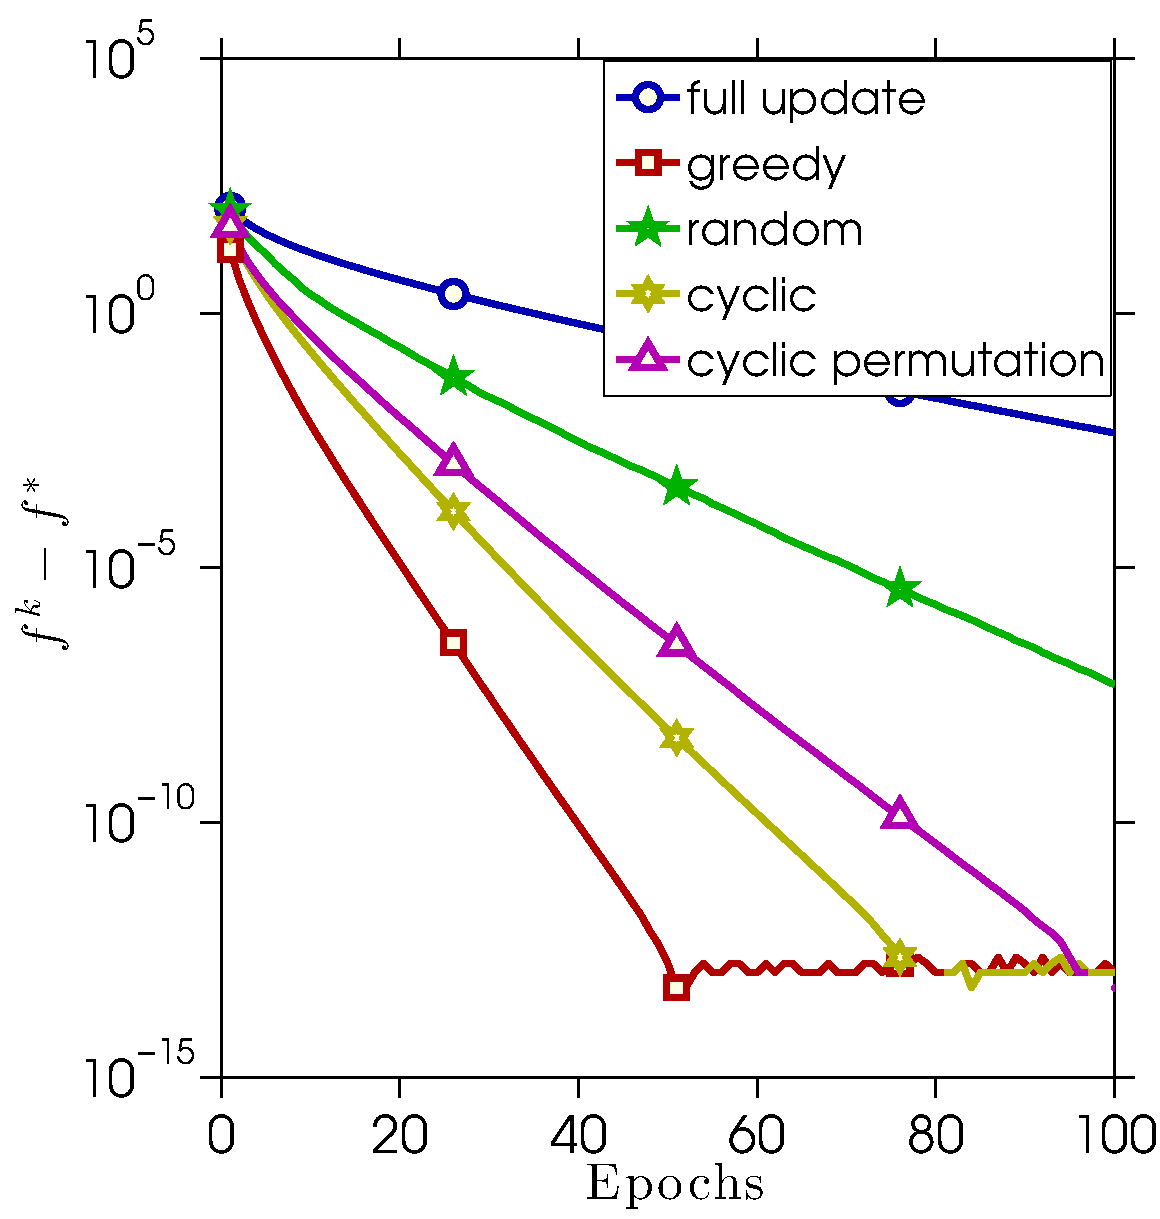
\includegraphics[width=50mm]{./figs/randn_matrix_cropped}

\caption{Gradient descent: the coordinate updates are faster than the full update since the former can take larger steps at each step.}
\label{fig:ls_full_vs_coord}
\end{figure}



\subsubsection{Parallel Update} As one of their main advantages, coordinate update algorithms are easy to parallelize. In this subsection, we discuss  both synchronous (sync) and asynchronous (async) parallel updates.

\textbf{Sync-parallel (Jacobi) update} specifies a sequence of index subsets $\II_1,\II_2,\ldots \subseteq \{1,\ldots,n\}$, and at each iteration $k$,  the coordinates in $\II_k$ are updated in parallel by multiple agents:
$$ \begin{cases}
x^{k+1}_{i} = x_{i}^k - \eta_k(x^k-\cT x^k)_{i},& i\in \II_k,\\
x^{k+1}_{i} = x_i^k,&i\not\in \II_k.
\end{cases}
$$
Synchronization across all agents ensures that  all $x_i$ in $\II_k$ are updated and also written to the memory before the next iteration starts. Note that, if $\II_k=\{1,\ldots,n\}$, then all the coordinates are updated and, thus, each iteration reduces to the full update: $x^{k+1} =  x^k - \eta_k(x^k-\cT x^k).$ \cut{\color{red}This, of course, does not mean solving $x=\cT x$ in one step; therefore, do not confuse performing an  update in \eqref{coordes} for all the coordinates in parallel from the joint minimization over all the variables.}

\textbf{Async-parallel update.} In this setting, a set of agents  still perform parallel updates, but synchronization is eliminated or weakened. Hence, each of them continuously applies \eqref{fm:async} below, which reads    $x$  from the shared memory and writes $x_i$ back (or through communicating without shared memory):  
\beq\label{fm:async} \begin{cases}
x^{k+1}_{i} = x_{i}^k - \eta_k \left((\cI-\cT) x^{k-d_k}\right)_{i},& i=i_k,\\
x^{k+1}_{i} = x_i^k,& \text{for all }i\not= i_k.
\end{cases}
\eeq
Unlike before, $k$ increases  whenever any agent completes an update. 

The lack of synchronization often results in computation with out-of-date information. During the computation of the $k$th update, other agents make $d_k$ updates to $x$ in the shared memory; when the $k$th update is written, its input is already $d_k$ iterations out of date. This number is  referred to as the the asynchronous delay. In~\eqref{fm:async}, the agent reads $x^{k-d_k}$ and commits the update to $x_{i_k}^k$. Here we have assumed  \emph{consistent} reading, i.e., $x^{k-d_k}$ lying in the set $\{x^j\}_{j=1}^k$. This requires implementing a memory lock. Removing the lock can lead to  \emph{inconsistent} reading, which still has convergence guarantees; see~\cite[Section 1.2]{Peng_2015_AROCK} for more details.


\begin{figure} \centering
    \begin{subfigure}[b]{0.45\linewidth}
        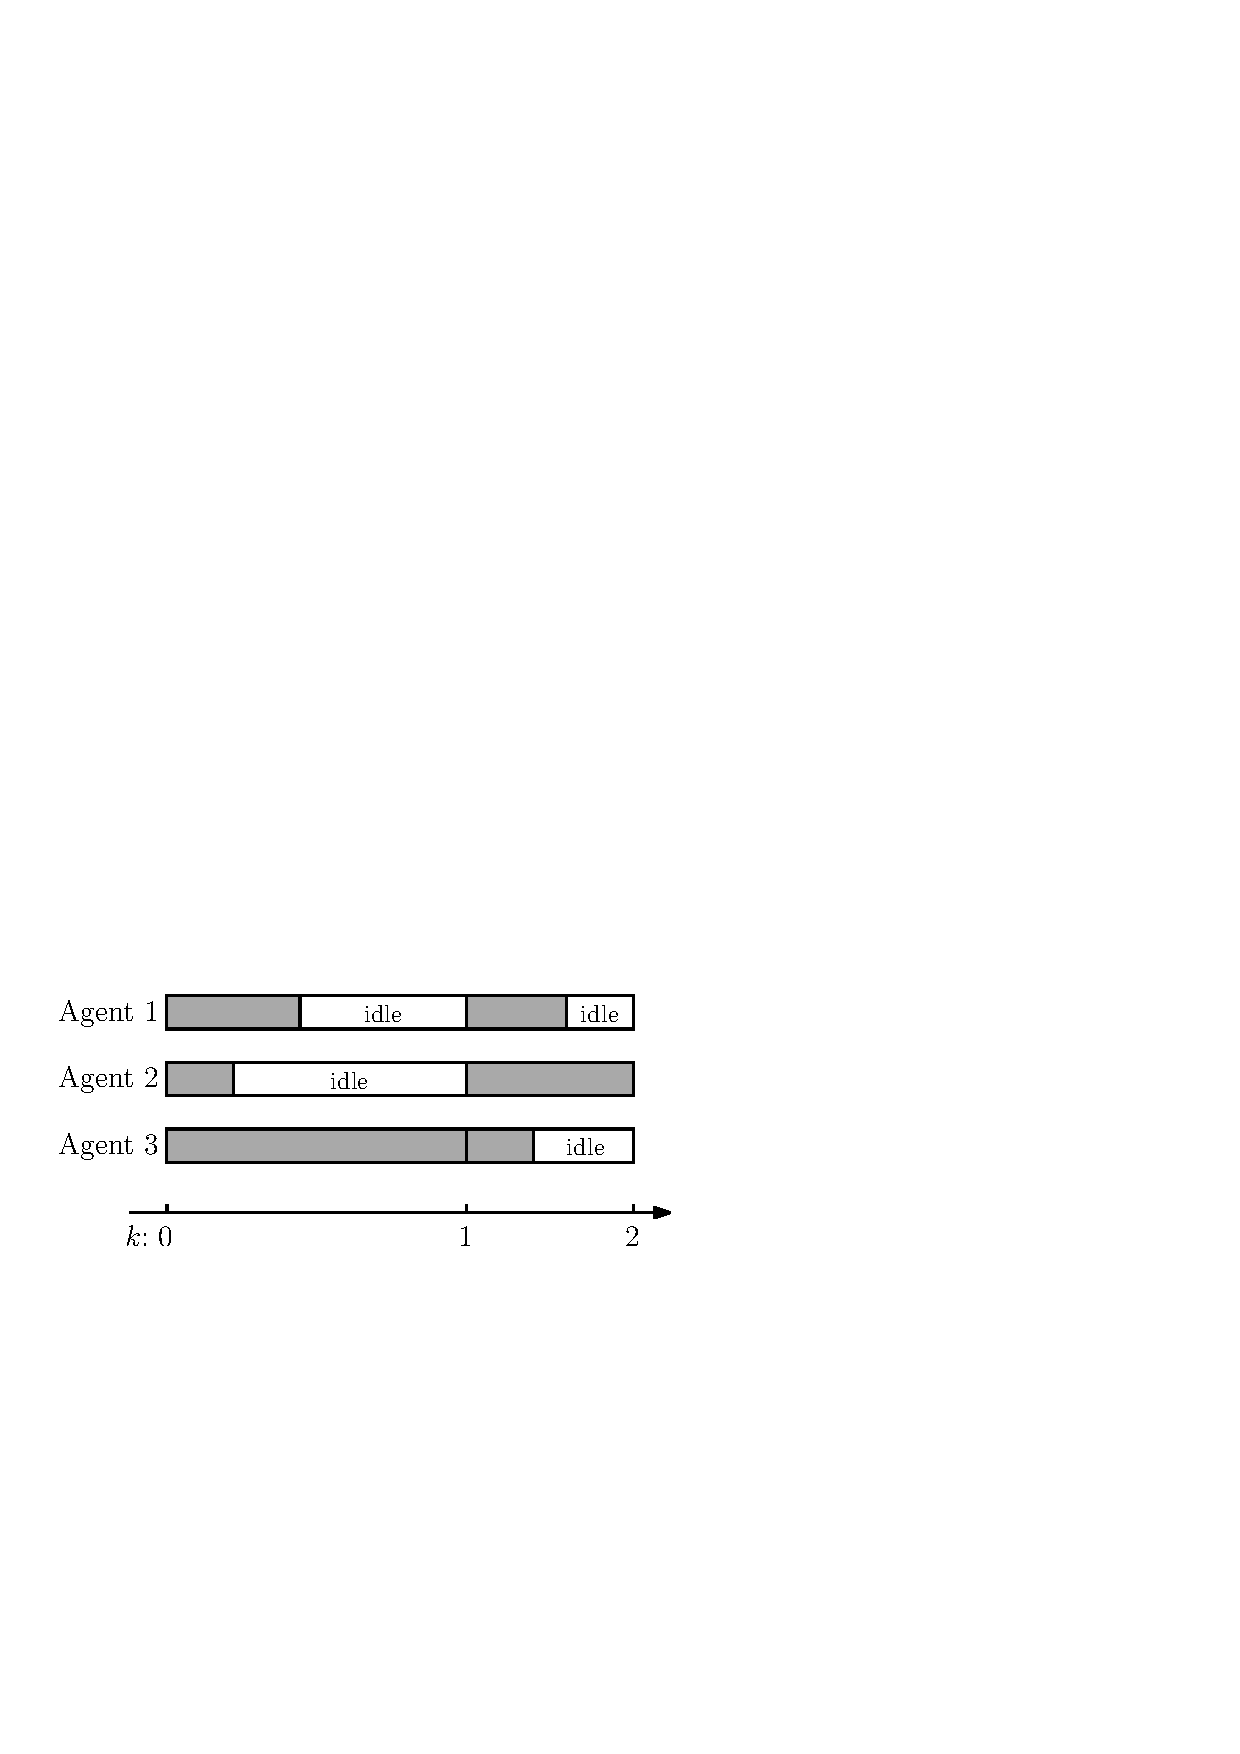
\includegraphics[width=60mm]{./figs/syn-simple}
        \caption{sync-parallel computing}
        \label{fig:parallel_a}
    \end{subfigure} %
    \quad
    \begin{subfigure}[b]{0.45\linewidth}
        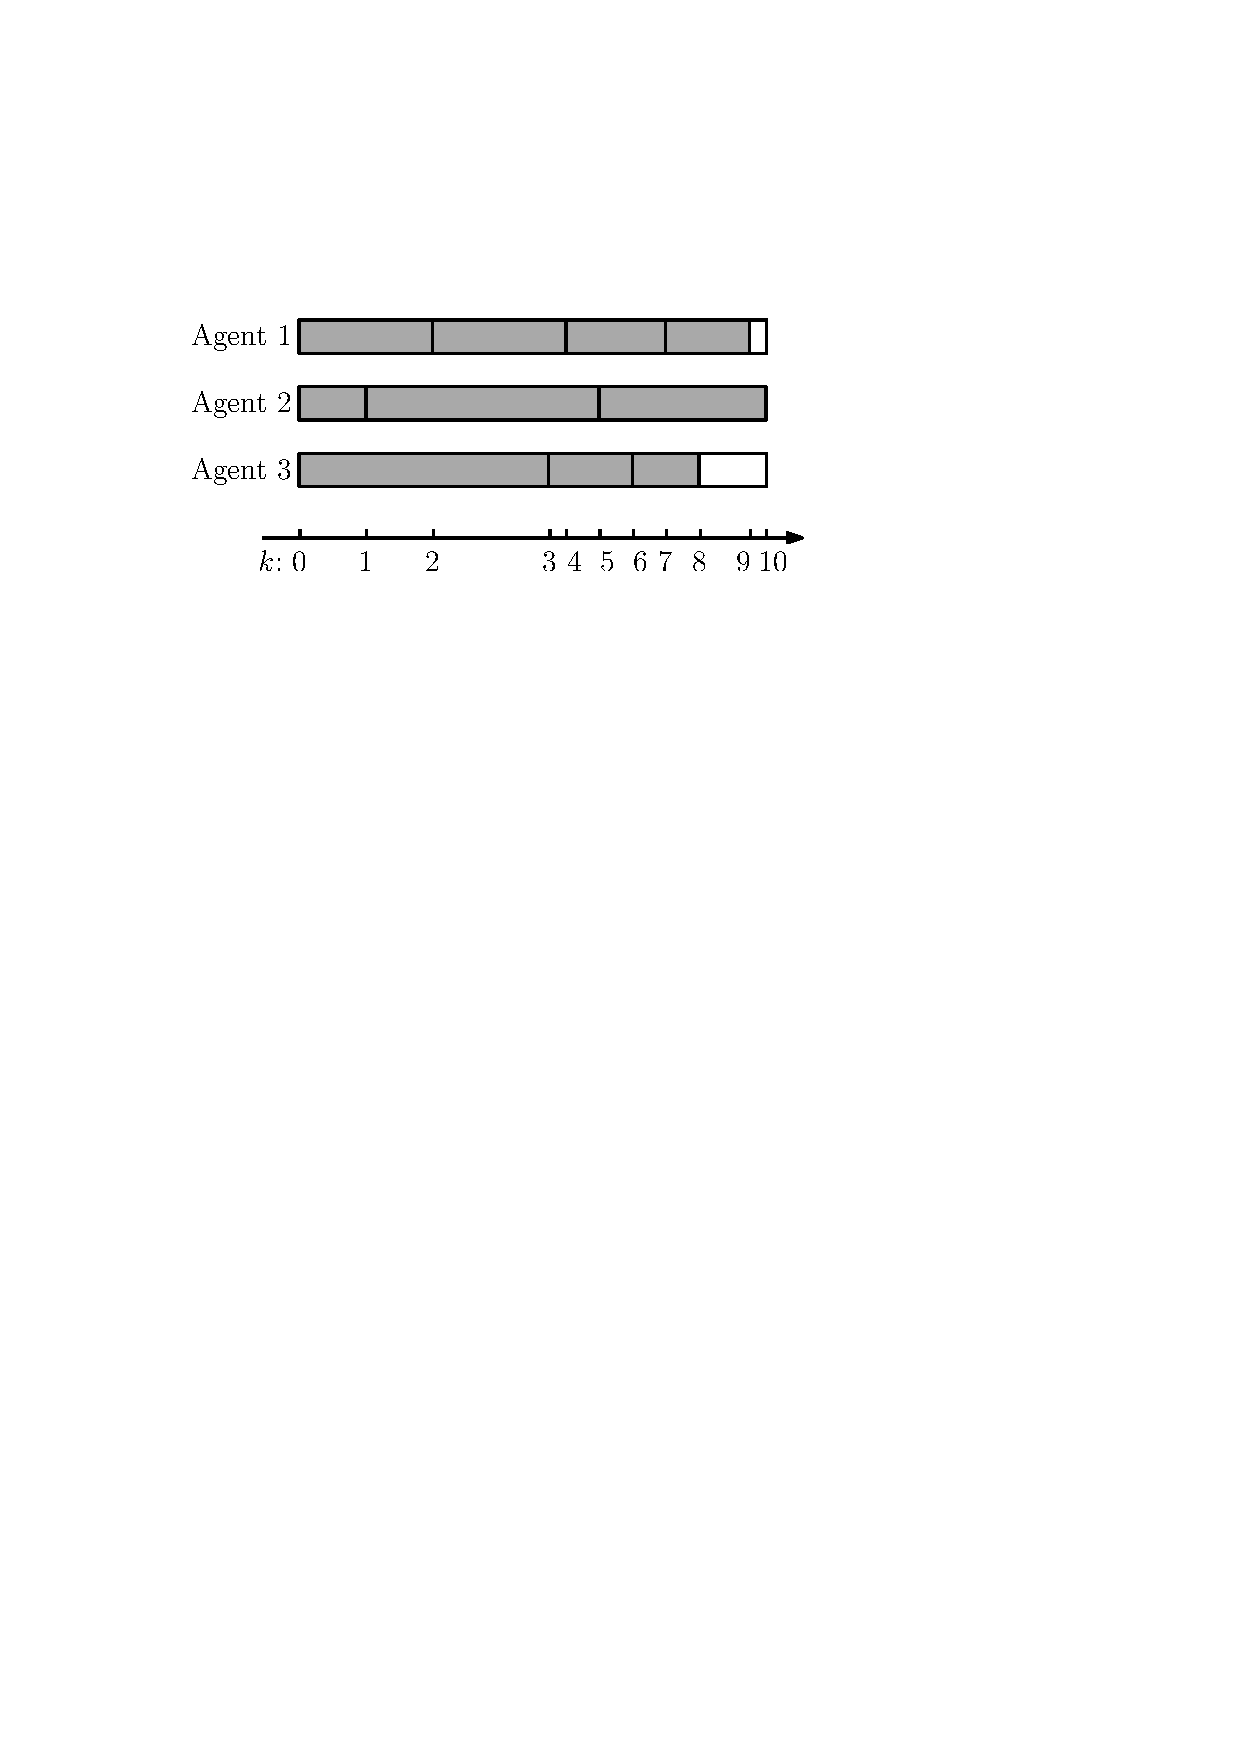
\includegraphics[width=60mm]{./figs/asyn-simple}
        \caption{async-parallel computing}
        \label{fig:parallel_b}
    \end{subfigure} %
    \caption{ Sync-parallel computing (left) versus async-parallel computing (right). On the left, all the agents must wait at idle (white boxes) until the slowest agent has finished.}
    \label{fig:comp_sync_async}
\end{figure}

% \begin{center}[picture: sync-parallel vs async-parallel]\end{center}

Synchronization across all agents means that all agents will wait for  the last (slowest) agent to complete. %It is not truly scalable since, as the number of agents increase, the slowest update  becomes slower and also because it is not fault tolerant. In addition, in the synchronous algorithm, all the processors simultaneously make congestion-inducing communication and memory-access requests.
Async-parallel updates eliminate such idle time, spread out memory access and  communication, and thus often run much faster.  However, async-parallel is more difficult to analyze because of the asynchronous delay.

%Asynchronous delay occurs if, after an agent reads $x$ yet before it completes updating $x_{i_k}$, other agents also make updates to $x$. 
%Here, $d_k$ is a scalar in the \emph{consistent} case and a vector in the \emph{atomically inconsistent} case. In the former case, the delays of the entries of $x^{k-d_k}$ are consistent, namely,  $x^{k-d_k}=[x^{k-d_k}_1,\ldots,x^{k-d_k}_n]$. \emph{Atomic inconsistency}, on the other hand, allows inconsistent delays: $x^{k-d_k}=[x^{k-d_{k,1}}_1,\ldots,x^{k-d_{k,n}}_n]$, where $d_k\in\NN^n$ is a vector and $n$ is the number of block coordinates. Inconsistency occurs when multiple agents read and write the entries of $x$ simultaneously, but  atomicity of $x_i$ ensures that all the sub-entries or bits of  $x_i$ are read and written at once and thus stay consistent.

\remove{The sync-parallel update is a special case of the async-parallel update where the number of agents equals $|\II_k|$ and  the asynchronous delay is uniformly zero.}

\textbf{Parallel-update literature.} 
Async-parallel methods can be traced back to~\cite{chazan1969chaotic} for linear systems. For function minimization,~\cite{bertsekas1989parallel} introduced an async-parallel gradient-projection method. Convergence rates are obtained in~\cite{tseng1991rate-asyn}.  
Recently, \cite{bradley2011parallel,richtarik2012parallel} developed parallel randomized methods. 

For fixed-point problems, async-parallel methods date back to~\cite{Baudet_1978_asynchronous} in 1978. In  the pre-2010 methods \cite{BMR1997asyn-multisplit,bertsekas1983distributed,Baz200591,el1998flexible} and the review~\cite{Frommer2000201}, each agent updates its own subset of coordinates. Convergence is established under the \emph{$P$-contraction} condition and its variants~\cite{bertsekas1983distributed}. Papers~\cite{Baz200591,Baz1998429} show convergence for async-parallel iterations with simultaneous reading and writing to the same set of components. Unbounded but stochastic delays are considered in~\cite{Strikwerda2002125}.

Recently, random coordinate selection appeared in~\cite{Patrick_2015} for fixed-point problems. The works \cite{nedic2001distributed,recht2011hogwild,liu2013asynchronous,liu2014asynchronous,hsieh2015passcode} introduced async-parallel stochastic methods for function minimization.
For fixed-point problems,~\cite{Peng_2015_AROCK} introduced  async-parallel stochastic methods, as well as several applications.  

\subsection{Contributions of this paper} 
The paper systematically discusses the CF properties found in both single and composite operators underlying many interesting applications. We introduce approaches to recognize CF operators and develop coordinate-update algorithms based on them. 
We provide a variety of applications to illustrate our approaches. 
In particular, we obtain new coordinate-update algorithms for image deblurring, portfolio optimization, second-order cone programming, as well as tensor decomposition. Our analysis also provides guidance to the implementation of coordinate-update algorithms by specifying how to compute certain operators and maintain certain quantities in memory. We also provide numerical results to illustrate the efficiency of the proposed coordinate update algorithms.
 
This paper does \emph{not} focus on the convergence perspective of coordinate update algorithms, though a convergence proof is provided in the appendix for a new primal-dual coordinate update algorithm. In general, in fixed-point algorithms, the iterate convergence is ensured by the monotonic decrease of the distance between the iterates and the solution set, while in minimization problems, the objective value convergence is ensured by the monotonic decrease of a certain energy function. The reader is referred to the existing literature for details. 

%{\color{red}In general, their convergence are ensured by a certain monotonically decreasing energy function in unconstrained minimization, giving  objective value convergence, and by the  monotonically decreasing distance to the solution set in fixed-point problems, giving point convergence (and objective value convergence if applied to minimization). }

%In our fixed-point setting, the operator $\cT$ generally needs to be  nonexpansive (under a certain metric). The operator splitting methods reviewed in~\S\ref{sec:comp-cuf} below generate nonexpansive operators $\cT$ for many problems considered in this paper. The convergence of the resulting stochastic sequential and  (async)-parallel coordinate-update algorithms, as well as their step size selections, is referred to the recent works~\cite{Patrick_2015,Peng_2015_AROCK}. On the other hand, 
The structural properties of operators discussed in this paper are irrelevant to  the convergence-related properties such as nonexpansiveness (for an operator) or convexity (for a set or function). Hence, the algorithms developed can be still applied to nonconvex problems.


%\end{subsection}

%\end{section}
% at solving large-sized problems involving  linear and nonlinear maps, and smooth and nonsmooth functions.  at solving large-sized problems involving  linear and nonlinear maps, and smooth and nonsmooth functions. 
 %DIF < \DIFdelbegin \DIFdel{It handles both  linear and nonlinear maps, and smooth and nonsmooth functions. The most common examples  }\DIFdelend %DIF > It handles both  linear and nonlinear maps, and smooth and nonsmooth functions. The most common examples 
